\documentclass{beamer}
\usetheme{Boadilla}

\usepackage[utf8]{inputenc}
\usepackage[french]{babel} %pour la typographie française.
\usepackage[T1]{fontenc} %pour la césure des mots.
\usepackage{amssymb} %pour les symboles mathématiques et lettres grecques
\usepackage{amsmath} %pour les formules mathématiques avancées

\beamertemplatenavigationsymbolsempty % Flag nazi pour supprimer la ligne d'option dans les slides

\title{Projet TriComp : Présentation}
\author{Equipe TriComp}
\date{Jeudi 18 Décembre 2014}

\begin{document}

\frame{
   \begin{center}
        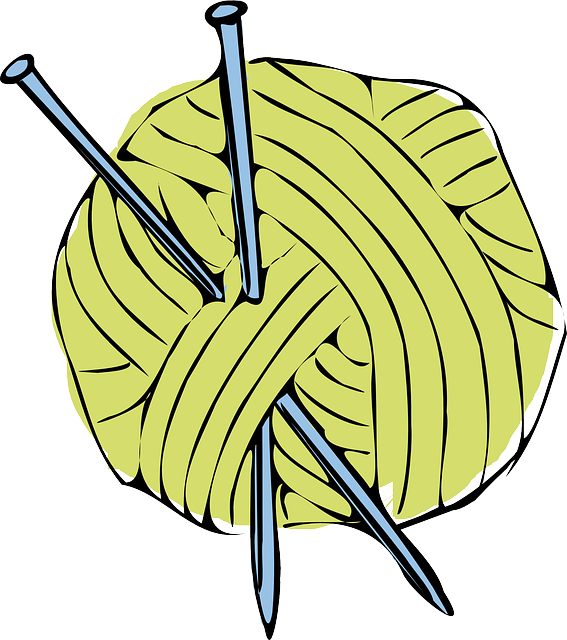
\includegraphics[height=0.2\textheight]{../img/ball_of_wool.png}
        \hspace*{4cm}
        
\includegraphics[height=0.2\textheight]{../img/ens.jpg}
   \end{center}
   \titlepage
}

\frame{
	\frametitle{L'équipe TriComp}
		\begin{center}
			{\large
			{William \textsc{Aufort} \hspace{4cm} Julien \textsc{Bensmail} \\}
			\vspace{1cm}
			{Agathe \textsc{Herrou}  \hspace{4cm} Romain \textsc{Labolle} \\}
			\vspace{1cm}
			{Frédéric \textsc{Lang} \hspace{4cm} Maxime \textsc{Lesourd} \\}
			\vspace{1cm}       
			{Laureline \textsc{Pinault} \hspace{3.7cm} Léo \textsc{Stéfanesco} \\}}
		\end{center}
}

\frame{
	\frametitle{Plan} 
		\tableofcontents
}

\section{Introduction}

\subsection{Présentation générale}

\frame{
	\frametitle{Présentation générale}
		% TriComp = Tricot + Compilateur
		% Tricot -> logiciel pour tricoteur
		% Compilateur -> réalisation du tricot
		% ==> Un logiciel d'édition de tricot, mais surtout de génération d'instructions 
}

\subsection{Motivations}

\frame{
	\frametitle{Motivations}
		% Logiciels de tricot actuels : beaucoup d'édition, mais 
		% Livre de tricot : difficiles à suivre ? Pas spécifique à une pièce en particulier.
		% Originalité.		
		% Autres ...
}

\frame{
	\frametitle{Quelques notions de tricot...}
}

% Proposition de plan :
% Introduction : présentation de l'équipe, 
% TriComp : Origine de l'idée, Compilateur ? Tricot ?
% Travail en amont : Problèmes à résoudre (allocation aiguilles, qqchose de général) -> "langage haut niveau"
% Coté logiciel : interface
% Difficultés rencontrées
% Améliorations possibles (complexifier fonctionnalites, reprendre les objectifs non traités du midterm)

\end{document}

